\documentclass[a4paper,11pt]{report}
\usepackage[T1]{fontenc}
\usepackage[utf8]{inputenc}
\usepackage[francais]{babel}
\usepackage[usenames,dvipsnames,svgnames,table]{xcolor}
\usepackage[colorlinks,linkcolor={blue!30!black},citecolor={blue!50!black},urlcolor={blue!80!black}]{hyperref}
\usepackage{amsmath,amsfonts,array,graphicx,caption,lmodern,subcaption,tikz,url,xspace,wrapfig}
\usepackage{textcomp,rotating,epic,eepic,pdfpages,pgfplots,listings}
\usepackage[top=2cm,left=2.5cm,right=2.5cm,bottom=2cm]{geometry}
\usepackage[babel=true,kerning=true]{microtype}
\usepackage{float}
\parskip=6pt % adds vertical space between paragraphs

\lstset
{
    breaklines=true,
    tabsize=3,
    showstringspaces=false
}
\lstdefinestyle{Common}
{
    extendedchars=\true,
    language={[Visual]Basic},
    frame=single,
    %===========================================================
    framesep=3pt,%expand outward.
    framerule=0.4pt,%expand outward.
    xleftmargin=3.4pt,%make the frame fits in the text area. 
    xrightmargin=3.4pt,%make the frame fits in the text area.
    %=========================================================== 
    rulecolor=\color{Red!0},
    backgroundcolor=\color{Yellow!10},
    basicstyle=\tiny\color{Black}\ttfamily,
    keywordstyle=\color{Orange},
    identifierstyle=\color{Blue},
    stringstyle=\color{Red},
    commentstyle=\color{Green}
}


\begin{document}

\pagenumbering{gobble}  % Pas de numérotation
\begin{titlepage}
    \vspace*{50px}
    
\includegraphics[height=80px]{Images/logo_phelma.pdf}
    \vspace*{-80px}
\begin{flushright}
%     \vspace*{60px}
    
\includegraphics[height=65px]{Images/CIME.jpg}
\end{flushright}

\vspace*{2cm}

\begin{center}
\rule{\linewidth}{0.5mm}\\[0.4cm]
{\huge{\bfseries Compte Rendu}\\[0.4cm]
\textsc{TP Simulation électronique}\\[0.4cm]}
\rule{\linewidth}{0.5mm}\\[0.5cm]

\LARGE{\textsc{Nicolas Paillet, Félix Piédallu \& Giulia Rizzo}}\\[0.7cm]
\large{\textsc{2015-2016}}\\[2cm]

\Large{~}\\[1cm]
% 
\includegraphics[width=0.4\textwidth]{Images/CIME.jpg}\\[1cm]
%
 \large{Encadrant : Marco Pala}\\[2cm]
%

\end{center}
\end{titlepage}

\tableofcontents        % Table des matières avec liens, générée automatiquement.
\newpage
\pagenumbering{arabic}  % Numérotation de retour !


\chapter*{Introduction}
\addcontentsline{toc}{chapter}{Introduction}

L'essor des télécommunications optiques n'est désormais plus à prouver. Omniprésentes dans la plupart des réseaux de télécommunication, les fibres optiques sont devenues incontournables. Elles sont d'autant plus intéressantes qu'il est possible de véhiculer plusieurs signaux dans une seule et même fibre, à différentes longueurs d'ondes. \newline
Il est alors nécessaire de pouvoir séparer en fin de fibre les différentes longueurs d'onde, d'où l'utilisation de démultiplexeurs.

Le but de ce bureau d'étude est de simuler le fonctionnement d'un coupleur directionnel et de mesurer ses performances pour le démultiplexage de deux longueur d'ondes.

Nous mettrons en évidence les différents paramètres que l'on peut adapter pour modifier le fonctionnement du composant, tels que les indices effectifs $n_{eff}$, la distance entre les deux guides et la longueur du coupleur.
\newline
\indent Nous mesurerons enfin les performances du démultiplexeur, illustrées par l'isolation des deux bras aux longueurs d'ondes nominales de fonctionnement, ainsi que la tolérance en longueur d'onde du fonctionnement du dispositif et les effets de la courbure en entrée et sortie du coupleur.


\chapter{Étude théorique}

\section{Présentation du démultiplexeur}
\begin{figure}[H]
    \begin{center}
        \definecolor{c0079ff}{RGB}{0,121,255}
\definecolor{c11de00}{RGB}{17,222,0}
\definecolor{cff0000}{RGB}{255,0,0}


\begin{tikzpicture}[y=0.80pt, x=0.80pt, yscale=-0.300000, xscale=0.300000, inner sep=0pt, outer sep=0pt]
\begin{scope}[cm={{1.0,0.0,0.0,0.66472,(0.0,513.65009)}}]% layer1-3
  % path4152-9
  \draw(60,230)node[above, scale = 1.3]{\color{c11de00}$\lambda_1$,\color{cff0000}$\lambda_2$};
  \path[draw=c0079ff,line join=miter,line cap=butt,miter limit=4.00,even odd rule,line width=5.000pt]
    (1200.0000,250.0000) .. controls (1000.0000,250.0000) and (1000.0000,400.0000) .. (800.0000,400.0000) --
    (400.0000,400.0000)  .. controls  (200.0000,400.0000) and  (200.0000,250.0000) .. (0.0000,250.0000);

  % path4152-3-7
  \path[draw=c0079ff,line join=miter,line cap=butt,miter limit=4.00,even odd rule,line width=5.000pt]
    (1200.0000,600.0000) .. controls (1000.0000,600.0000) and (1000.0000,450.0000) .. (800.0000,450.0000) --
    (400.0000,450.0000)  .. controls  (200.0000,450.0000) and  (200.0000,600.0000) .. (0.0000,600.0000);

  \draw(1200,230)node[above, scale = 1.3]{\color{c11de00}$\lambda_1$};
  % path4700
  \path[draw=c11de00,line width=2.000pt,->]
    (390.0000,400.0000) .. controls (498.9497,400.0000) and (503.3310,450.0000) ..
    (600.0000,450.0000) .. controls (696.6690,450.0000) and (736.6388,400.0000) .. (810.0000,400.0000);

  \draw(1200,710)node[above, scale = 1.3]{\color{cff0000}$\lambda_2$};
  % path4990
  \path[draw=cff0000,line width=2.000pt,->]
    (390.0000,400.0000) .. controls (665.7450,400.0000) and (506.9814,450.0000) .. (810.0000,450.0000);

\end{scope}

\end{tikzpicture}

        \caption{Schéma de principe du démultiplexeur}
        \label{fig:}
    \end{center}
\end{figure}

Le dispositif du coupleur est constitué de deux guides linéaires de longueur \textbf{L}, espacés d'une distance \textbf{d}.

Quatre bras en "S" permettent la connexion de ces deux guides aux fibres d'entrée et de sortie.
L'intégralité du signal provient d'un seul bras (haut-gauche), aux deux longueurs d'onde $\lambda_1$ et $\lambda_2$.

On souhaite que l'intégralité du signal à $\lambda_1$ sorte par le haut et le signal à $\lambda_2$, par le bas.

Ce problème peut alors être vu selon deux approches, que nous allons détailler.

\section{Approche perturbative}
Un guide propage la puissance lumineuse, mais il existe aussi une partie évanescente hors du guide.

Dans le cas d'un guide isolé, on n'observe pas de pertes dues à cette partie évanescente.

Le rajout d'un second guide est alors perçu comme une perturbation par le premier guide : la partie évanescente est captée par le second guide, d'où l'apparition de puissance. La totalité de la puissance présente dans le premier guide sera transférée dans le second guide, qui va alors lui-même subir une perturbation par le premier guide.

On observe donc un couplage entre les deux guides, et la puissance dans chacun des guides suivra une loi sinusoïdale dans la direction de propagation.

Plus la distance d entre les deux guides est élevée, plus le transfert de puissance sera long : la partie évanescente captée par le second guide décroît en $e^{-d^2}$.

On peut donc déjà définir la longueur de couplage $L_c$, longueur nécessaire pour un transfert total de la puissance d'un guide à l'autre.

\section{Approche globale}%TODO nom à améliorer
Une autre approche consiste à considérer les deux guides comme une seule superstructure, et les deux modes fondamentaux de propagation pair et impair, comme le montre la figure \ref{schema_modes}
\begin{figure}[H]
    \begin{center}
        \definecolor{c0079ff}{RGB}{0,121,255}
\definecolor{c11de00}{RGB}{17,222,0}
\definecolor{cff0000}{RGB}{255,0,0}


\begin{tikzpicture}[y=0.80pt, x=0.80pt, yscale=-0.300000, xscale=0.300000, inner sep=0pt, outer sep=0pt]
\begin{scope}[shift={(0,-343.70079)}]% layer1
  \begin{scope}[shift={(0,292.3622)}]% layer1-3
  % path4152-9
  \draw(60,230)node[above, scale = 1.3]{\color{c11de00}$\lambda_1$,\color{cff0000}$\lambda_2$};
  \path[draw=c0079ff,line join=miter,line cap=butt,miter limit=4.00,even odd rule,line width=5.000pt]
    (1200.0000,250.0000) .. controls (1000.0000,250.0000) and (1000.0000,400.0000) .. (800.0000,400.0000) --
    (400.0000,400.0000)  .. controls  (200.0000,400.0000) and  (200.0000,250.0000) .. (0.0000,250.0000);y

  % path4152-3-7
  \path[draw=c0079ff,line join=miter,line cap=butt,miter limit=4.00,even odd rule,line width=5.000pt]
    (1200.0000,600.0000) .. controls (1000.0000,600.0000) and (1000.0000,450.0000) .. (800.0000,450.0000) --
    (400.0000,450.0000)  .. controls  (200.0000,450.0000) and  (200.0000,600.0000) .. (0.0000,600.0000);

  \draw(1200,230)node[above, scale = 1.3]{\color{c11de00}$\lambda_1$};
  % path4700
  \path[draw=c11de00,line width=2.000pt,->]
    (390.0000,400.0000) .. controls (498.9497,400.0000) and (503.3310,450.0000) ..
    (600.0000,450.0000) .. controls (696.6690,450.0000) and (736.6388,400.0000) .. (810.0000,400.0000);

  \draw(1200,710)node[above, scale = 1.3]{\color{cff0000}$\lambda_2$};
  % path4990
  \path[draw=cff0000,line width=2.000pt,->]
    (390.0000,400.0000) .. controls (665.7450,400.0000) and (506.9814,450.0000) .. (810.0000,450.0000);

  \end{scope}
  \begin{scope}[shift={(-362.80972,149.87023)}]% g5587
    \begin{scope}[cm={{0.32005,0.0,0.0,0.48585,(270.86169,136.38442)}}]% g4421-7
      \begin{scope}[cm={{0.0,1.0,-1.0,0.0,(1501.0978,350.7074)}}]% g4484
        \begin{scope}[shift={(-43.38739,-35.32403)}]% g5548
          % path4371-9
          \path[draw=c11de00,line join=miter,line cap=round,miter limit=4.00,nonzero
            rule,line width=0.700pt] (407.5099,985.2193) .. controls (423.4799,985.1873)
            and (439.4500,947.0765) .. (455.4200,912.2461) .. controls (471.3900,877.4156)
            and (487.3601,856.2800) .. (503.3301,871.7490) .. controls (519.3001,887.2179)
            and (535.2701,934.7990) .. (551.2402,962.7451) .. controls (567.2102,990.6913)
            and (583.1802,990.6513) .. (599.1503,962.7451) .. controls (615.1203,934.8390)
            and (631.0903,887.2757) .. (647.0604,871.7490) .. controls (663.0304,856.2222)
            and (679.0004,877.4299) .. (694.9704,912.2461) .. controls (710.9405,947.0623)
            and (726.9105,985.1873) .. (742.8805,985.2193);

          % path4414-0
          \path[draw=black,line join=miter,line cap=round,miter limit=4.00,even odd
            rule,line width=0.700pt] (407.5917,985.2188) -- (742.4380,985.2087);

        \end{scope}
      \end{scope}
    \end{scope}
    \begin{scope}[cm={{0.0,1.01795,-0.69903,0.0,(1066.9692,102.71188)}}]% g5552
      % path5513
      \path[draw=c11de00,line join=miter,line cap=round,miter limit=4.00,nonzero
        rule,line width=0.700pt] (374.0981,950.3649) .. controls (381.7166,950.3649)
        and (389.3351,942.6874) .. (396.9536,923.3599) .. controls (404.5721,904.0324)
        and (412.1906,887.2935) .. (419.8092,898.0022) .. controls (427.4277,908.7109)
        and (435.0462,937.1323) .. (442.6647,945.7493) .. controls (450.2832,954.3663)
        and (457.9017,946.3918) .. (465.5202,954.9804) .. controls (473.1387,963.5691)
        and (480.7572,991.9811) .. (488.3757,1002.7276) .. controls
        (495.9942,1013.4741) and (503.6127,996.7033) .. (511.2312,977.3699) ..
        controls (518.8497,958.0365) and (526.4683,950.3649) .. (534.0868,950.3649);

      % path5546
      \path[draw=black,line join=miter,line cap=round,miter limit=4.00,even odd
        rule,line width=0.700pt] (374.0981,950.3649) -- (534.0868,950.3649);

    \end{scope}
  \end{scope}
  \begin{scope}[shift={(-225.6667,-161.58773)}]% g5597
    \begin{scope}[cm={{0.0,0.48671,-0.32003,0.0,(754.88477,596.80337)}}]% g4421
      \begin{scope}% g4462
        % path4371
        \path[draw=cff0000,line join=miter,line cap=round,miter limit=4.00,nonzero
          rule,line width=0.700pt] (407.5099,985.2193) .. controls (423.4799,985.1873)
          and (439.4500,947.0765) .. (455.4200,912.2461) .. controls (471.3900,877.4156)
          and (487.3601,856.2800) .. (503.3301,871.7490) .. controls (519.3001,887.2179)
          and (535.2701,934.7990) .. (551.2402,962.7451) .. controls (567.2102,990.6913)
          and (583.1802,990.6513) .. (599.1503,962.7451) .. controls (615.1203,934.8390)
          and (631.0903,887.2757) .. (647.0604,871.7490) .. controls (663.0304,856.2222)
          and (679.0004,877.4299) .. (694.9704,912.2461) .. controls (710.9405,947.0623)
          and (726.9105,985.1873) .. (742.8805,985.2193);

        % path4414
        \path[draw=black,line join=miter,line cap=round,miter limit=4.00,even odd
          rule,line width=0.700pt] (407.5917,985.2188) -- (742.4380,985.2087);

      \end{scope}
    \end{scope}
    \begin{scope}[cm={{0.0,1.01795,-0.69903,0.0,(1061.0833,414.58936)}}]% g5552-2
      \begin{scope}[shift={(0,2.86111)}]% g5583
        % path5513-8
        \path[draw=cff0000,line join=miter,line cap=round,miter limit=4.00,nonzero
          rule,line width=0.700pt] (374.0981,950.3649) .. controls (381.7166,950.3649)
          and (389.3351,942.6874) .. (396.9536,923.3599) .. controls (404.5721,904.0324)
          and (412.1906,887.2935) .. (419.8092,898.0022) .. controls (427.4277,908.7109)
          and (435.0462,937.1323) .. (442.6647,945.7493) .. controls (450.2832,954.3663)
          and (457.9017,946.3918) .. (465.5202,954.9804) .. controls (473.1387,963.5691)
          and (480.7572,991.9811) .. (488.3757,1002.7276) .. controls
          (495.9942,1013.4741) and (503.6127,996.7033) .. (511.2312,977.3699) ..
          controls (518.8497,958.0365) and (526.4683,950.3649) .. (534.0868,950.3649);

        % path5546-7
        \path[draw=black,line join=miter,line cap=round,miter limit=4.00,even odd
          rule,line width=0.700pt] (374.0981,950.3649) -- (534.0868,950.3649);

      \end{scope}
    \end{scope}
  \end{scope}
  \begin{scope}[shift={(586.97911,150.0493)}]% g5587-1
    \begin{scope}[cm={{0.32005,0.0,0.0,0.48585,(270.86169,136.38442)}}]% g4421-7-7
      \begin{scope}[cm={{0.0,1.0,-1.0,0.0,(1501.0978,350.7074)}}]% g4484-7
        \begin{scope}[shift={(-43.38739,-35.32403)}]% g5548-9
          % path4371-9-2
          \path[draw=c11de00,line join=miter,line cap=round,miter limit=4.00,nonzero
            rule,line width=0.700pt] (407.5099,985.2193) .. controls (423.4799,985.1873)
            and (439.4500,947.0765) .. (455.4200,912.2461) .. controls (471.3900,877.4156)
            and (487.3601,856.2800) .. (503.3301,871.7490) .. controls (519.3001,887.2179)
            and (535.2701,934.7990) .. (551.2402,962.7451) .. controls (567.2102,990.6913)
            and (583.1802,990.6513) .. (599.1503,962.7451) .. controls (615.1203,934.8390)
            and (631.0903,887.2757) .. (647.0604,871.7490) .. controls (663.0304,856.2222)
            and (679.0004,877.4299) .. (694.9704,912.2461) .. controls (710.9405,947.0623)
            and (726.9105,985.1873) .. (742.8805,985.2193);

          % path4414-0-0
          \path[draw=black,line join=miter,line cap=round,miter limit=4.00,even odd
            rule,line width=0.700pt] (407.5917,985.2188) -- (742.4380,985.2087);

        \end{scope}
      \end{scope}
    \end{scope}
    \begin{scope}[cm={{0.0,1.01795,-0.69903,0.0,(1066.9692,102.71188)}}]% g5552-8
      % path5513-6
      \path[draw=c11de00,line join=miter,line cap=round,miter limit=4.00,nonzero
        rule,line width=0.700pt] (374.0981,950.3649) .. controls (381.7166,950.3649)
        and (389.3351,942.6874) .. (396.9536,923.3599) .. controls (404.5721,904.0324)
        and (412.1906,887.2935) .. (419.8092,898.0022) .. controls (427.4277,908.7109)
        and (435.0462,937.1323) .. (442.6647,945.7493) .. controls (450.2832,954.3663)
        and (457.9017,946.3918) .. (465.5202,954.9804) .. controls (473.1387,963.5691)
        and (480.7572,991.9811) .. (488.3757,1002.7276) .. controls
        (495.9942,1013.4741) and (503.6127,996.7033) .. (511.2312,977.3699) ..
        controls (518.8497,958.0365) and (526.4683,950.3649) .. (534.0868,950.3649);

      % path5546-72
      \path[draw=black,line join=miter,line cap=round,miter limit=4.00,even odd
        rule,line width=0.700pt] (374.0981,950.3649) -- (534.0868,950.3649);

    \end{scope}
  \end{scope}
  \begin{scope}[shift={(724.12212,-161.40866)}]% g5597-9
    \begin{scope}[cm={{0.0,0.48671,-0.32003,0.0,(754.88477,596.80337)}}]% g4421-1
      \begin{scope}% g4462-5
        % path4371-8
        \path[draw=cff0000,line join=miter,line cap=round,miter limit=4.00,nonzero
          rule,line width=0.700pt] (407.5099,985.2193) .. controls (423.4799,985.1873)
          and (439.4500,947.0765) .. (455.4200,912.2461) .. controls (471.3900,877.4156)
          and (487.3601,856.2800) .. (503.3301,871.7490) .. controls (519.3001,887.2179)
          and (535.2701,934.7990) .. (551.2402,962.7451) .. controls (567.2102,990.6913)
          and (583.1802,990.6513) .. (599.1503,962.7451) .. controls (615.1203,934.8390)
          and (631.0903,887.2757) .. (647.0604,871.7490) .. controls (663.0304,856.2222)
          and (679.0004,877.4299) .. (694.9704,912.2461) .. controls (710.9405,947.0623)
          and (726.9105,985.1873) .. (742.8805,985.2193);

        % path4414-9
        \path[draw=black,line join=miter,line cap=round,miter limit=4.00,even odd
          rule,line width=0.700pt] (407.5917,985.2188) -- (742.4380,985.2087);

      \end{scope}
    \end{scope}
    \begin{scope}[cm={{0.0,1.01795,-0.69903,0.0,(1061.0833,414.58936)}}]% g5552-2-7
      \begin{scope}[cm={{1.0,0.0,0.0,-1.0,(0.0,1903.6066)}}]% g5583-7
        % path5513-8-4
        \path[draw=cff0000,line join=miter,line cap=round,miter limit=4.00,nonzero
          rule,line width=0.700pt] (374.0981,950.3649) .. controls (381.7166,950.3649)
          and (389.3351,942.6874) .. (396.9536,923.3599) .. controls (404.5721,904.0324)
          and (412.1906,887.2935) .. (419.8092,898.0022) .. controls (427.4277,908.7109)
          and (435.0462,937.1323) .. (442.6647,945.7493) .. controls (450.2832,954.3663)
          and (457.9017,946.3918) .. (465.5202,954.9804) .. controls (473.1387,963.5691)
          and (480.7572,991.9811) .. (488.3757,1002.7276) .. controls
          (495.9942,1013.4741) and (503.6127,996.7033) .. (511.2312,977.3699) ..
          controls (518.8497,958.0365) and (526.4683,950.3649) .. (534.0868,950.3649);

        % path5546-7-6
        \path[draw=black,line join=miter,line cap=round,miter limit=4.00,even odd
          rule,line width=0.700pt] (374.0981,950.3649) -- (534.0868,950.3649);

      \end{scope}
    \end{scope}
  \end{scope}
\end{scope}

\end{tikzpicture}

        \caption{Schéma du multiplexeur avec les modes propagés}
        \label{schema_modes}
    \end{center}
\end{figure}


\subsection*{Considérons $\lambda_1$ (en vert).}
À l'entrée, les modes pair et impair sont en phase dans le guide supérieur (puissance maximale), et en opposition de phase dans le guide inférieur (pas de puissance).

Les deux modes ne sont pas soumis au même indice effectif $n_{eff}$, et ne se propagent donc pas à la même vitesse dans le dispositif.

En $L_c$, on se retrouve alors donc dans la situation opposée :
\begin{itemize}
    \item Opposition de phase dans le guide supérieur, et donc pas de puissance
    \item En phase dans le guide inférieur, avec une puissance maximale.
    \newline
\end{itemize}

On retrouve alors, comme dans la première approche, un couplage entre les deux guides, avec une puissance sinusoïdale dans les deux guides.


\subsection*{Dans le cas de $\lambda_2$ (en rouge),}
On retrouve exactement le même comportement ; $n_{eff}$ sera néanmoins différent, d'où une longueur de couplage ${L_c}_2$ différente.
\newline

L'approche perturbative est très bonne qualitativement, mais la seconde nous permettra d'étudier quantitativement le problème.

On calcule $L_c$ à partir des indices effectifs des deux modes, et en particulier de leur différence, car c'est la distance que mettent ces deux modes à se retrouver en opposition de phase, donc la distance de transfert du guide "haut" au guide "bas".

\begin{equation}
    L_c=\dfrac{\lambda}{2(n_{eff_p}-n_{eff_i})}
\end{equation}

\section{Position du problème}

Le but du multiplexeur est de séparer les longueurs d'onde, on en déduit ainsi qu'une relation permettant de séparer les longueurs d'onde est :
\begin{equation}
    2m\times{L_c}_1=(2p+1)\times{L_c}_2\,\,\hspace{1cm}\text{   avec m et p entiers}
\end{equation}

En effet, en $2m\times{L_c}_1$, la puissance associée à la longueur d'onde 1 fait m aller-retours et se retrouve dans le guide "haut", et en $(2p+1)\times{L_c}_2$, la puissance associée à la longueur d'onde 2 fait p aller-retours et change de nouveau de guide pour terminer dans le guide "bas". Nos longueurs d'ondes sont ainsi séparées. Cependant, en pratique, les dispositifs ne sont pas parfaits. 


% On veut alors qu'à la longueur d'onde 1, la puissance fasse $n$ aller-retours, tandis qu'à la longueur d'onde 2 elle fasse $m$ aller-retours puis retourne dans le second guide.
%
% Le problème consiste alors à trouver :
% \[
% \left\{
%     \begin{array}{ll}
%         2n\times {L_c}_1 = (2m+1)\times {L_c}_2 = L_{totale}\\
%         n, m\in \mathbb{N}
%     \end{array}
% \right.
% \]
%
C'est pour cela que nous souhaitons également caractériser la qualité du démultiplexeur par l'isolation des deux guides de sortie.
L'isolation à une longueur d'onde donnée est définie par :
\[
    \text{Isolation}(\lambda) = 10 \log\frac{P_{haut}(\lambda)}{P_{bas}(\lambda)}
\]
Où $P_{haut}$ et $P_{bas}$ sont les puissances sortant par les guides.

Cette formule nous donne des valeurs positives pour la longueur d'onde 1, et négatives pour la longueur d'onde 2. Le but du dispositif est d'avoir la meilleure isolation possible, pour séparer correctement les longueurs d'onde.

\chapter{Dimensionnement}
Afin de pouvoir étudier correctement les comportements de la structure que l'on souhaite étudier, il est important de dimensionner les guides correctement.

\section{Épaisseur des guides}
Nous avons étudié la théorie dans la partie précédente, il faut maintenant la mettre en application afin de déterminer les paramètres de fonctionnement optimaux. Ainsi, dans toute la suite, nous utiliserons les longueurs d'onde de fonctionnement suivantes :
\begin{itemize}
    \item $\lambda_1=1.55\mu m$ 
    \item $\lambda_2=1.31\mu m$
\end{itemize}
Ainsi que des indices valant :
\begin{itemize}
    \item  $n_{sub}=n_{sup}=1.50$ pour le substrat et le superstrat
    \item  $n_{c}=1.51$ pour le cœur du guide.
    \newline
\end{itemize}

En utilisant la méthode de l'indice effectif, puis grâce à l'equation caractéristique :
\begin{equation}
    k_0e\sqrt{n_c^2-n_{\text{eff}}^2}-\arctan\left(\sqrt{\dfrac{n_{eff}^2-n_{sub}^2}{n_{c}^2-n_{\text{eff}}^2}}\right)-\arctan\left(\sqrt{\dfrac{n_{\text{eff}}^2-n_{sup}^2}{n_{c}^2-n_{eff}^2}}\right)=m\pi
\end{equation}

Avec $e$ l'épaisseur du guide, et $k_0=\dfrac{2\pi}{\lambda}$.

En considérant le minimum de l'indice effectif, on peut alors trouver une épaisseur de coupure pour le mode fondamental (m=0) et une épaisseur de coupure pour le mode suivant (m=1), et ce pour chacune des longueurs d'onde considérées.

Ainsi, on obtient, après résolution de l'équation caractéristique pour ces 4 cas, des valeurs limites pour l'épaisseur du guide. Parmis les valeurs possibles, nous avons choisi une épaisseur $e=3\mu m$ pour chacun des guides, qui sont ainsi monomodes pour les deux longueurs d'ondes que nous allons utiliser, ce qui est confirmé par le solveur de modes intégré au logiciel qui nous donne $n_{\text{eff}_{\lambda_1}}=1.5020053$ et $n_{\text{eff}_{\lambda_1}}=1.5032$, pour $e=3\mu m$.

\section{Longueur des guides}
Nous avons de prendre une distance $d=3\mu m$ entre les guides. Grâce au solveur de modes, nous pouvons déterminer aisément les indices effectifs, en réalisant la structure telle que dans le Chapitre 1, en considérant l'aspect global.

\begin{figure}[H]
\centering
\begin{tikzpicture}
    \draw (7.5,-0.5) node{$n_{sub}=1.50$}; 
    \draw [thick](0,0)--(15,0);
    \draw (7.5,0.5) node{$n_c=1.51$};
    \draw [thick](0,1)--(15,1);
    \draw (7.5,1.5) node{ $n_{sub}=1.50$};
    \draw [thick](0,2)--(15,2);
    \draw (7.5,2.5) node{$n_c=1.51$};
    \draw [thick](0,3)--(15,3);
    \draw (7.5,3.5) node{$n_{sub}=1.50$}; 
    \draw [->](2,2.5)--(4,2.5)node[midway,below]{Sens de propagation};
    \path[fill=blue,opacity=0.05](0,-1)-- (15,-1)-- (15,4) -- (0,4) -- cycle;
    \path[fill=blue,opacity=0.2] (0,0) -- (15,0) -- (15,1) -- (0,1) -- cycle;
    \path[fill=blue,opacity=0.2] (0,2) -- (15,2) -- (15,3) -- (0,3) -- cycle;
\end{tikzpicture} 
\caption{Schéma de la structure réalisée dans le solveur de modes}

\end{figure}

\begin{description}
    \item[Pour $\lambda_1=1.55\,\mu m$,] le solveur nous donne
    \begin{itemize}
        \item $n_{\text{eff}1_p}=1.50574544$
        \item $n_{\text{eff}1_i}=1.50346926$
    \end{itemize}
    \item[Pour $\lambda_2=1.31\,\mu m$,] il nous donne
    \begin{itemize}
        \item $n_{\text{eff}2_p}=1.50620477$
        \item $n_{\text{eff}2_i}=1.50469404$
    \end{itemize}
\end{description}

On obtient alors pour $\lambda_1$, $L_{c_1}=339\,\mu m$ et pour $\lambda_2$, $L_{c_2}=433\,\mu m$. Ces longueurs de couplages nous donnent ainsi des ordres de grandeur afin de déterminer les longueurs de guide à utiliser pour réaliser le demultiplexeur.

En effet, en prenant $2m=4$ et $2(p+1)=3$, on obtient deux résultats proches, pour une longueur totale $L_{totale}=1300\,\mu m$.

Il faut maintenant entrer ces paramètres dans le logiciel de simulation afin de vérifier la validité de ces calculs et d'extraire des paramètres intéressants.
\chapter{Simulation} 

L'éditeur de script intégré dans OptiBPM nous permet de faire varier les caractéristiques de notre dispositif facilement, pour étudier leur impact sur les performances du démultiplexage.

\begin{description}
    \item[On déclare les variables :] LongueurLignes sera la valeur initiale de longueur, que l'on va incrémenter par la suite
\begin{lstlisting}[style=Common]
option explicit
WGMgr.DeleteAll
InputPlaneMgr.DeleteAll


Dim EspacementLignes, LongueurLignes
EspacementLignes    = 5
LongueurLignes      = 650

Dim LongueurS, LargeurS
LongueurS   = 400
LargeurS    = 5

Dim LineWidth
LineWidth = "2"
\end{lstlisting}


    \item[On déclare les guides :]
\begin{lstlisting}[style=Common]
Dim LinearTop, LinearBot, SBendArcTopI, SBendArcTopO, SBendArcBotI, SBendArcBotO


Set LinearTop = WGMgr.CreateObj ( "WGLinear", "LinearTop" )
Set LinearBot = WGMgr.CreateObj ( "WGLinear", "LinearBot" )
Set SBendArcTopI = WGMgr.CreateObj ( "WGSBendArc", "SBendArcTopI" )
Set SBendArcTopO = WGMgr.CreateObj ( "WGSBendArc", "SBendArcTopO" )
Set SBendArcBotI = WGMgr.CreateObj ( "WGSBendArc", "SBendArcBotI" )
Set SBendArcBotO = WGMgr.CreateObj ( "WGSBendArc", "SBendArcBotO" )

LinearTop.SetProfileName       "guidecanal1"
LinearBot.SetProfileName       "guidecanal1"
SBendArcTopI.SetProfileName    "guidecanal1"
SBendArcTopO.SetProfileName    "guidecanal1"
SBendArcBotI.SetProfileName    "guidecanal1"
SBendArcBotO.SetProfileName    "guidecanal1"

LinearTop.SetDefaultThicknessTaperMode     True
LinearBot.SetDefaultThicknessTaperMode     True
SBendArcTopI.SetDefaultThicknessTaperMode  True
SBendArcTopO.SetDefaultThicknessTaperMode  True
SBendArcBotI.SetDefaultThicknessTaperMode  True
SBendArcBotO.SetDefaultThicknessTaperMode  True

LinearTop.SetAttr      "WidthExpr", cstr(LineWidth)
LinearBot.SetAttr      "WidthExpr", cstr(LineWidth)
SBendArcTopI.SetAttr   "WidthExpr", cstr(LineWidth)
SBendArcTopO.SetAttr   "WidthExpr", cstr(LineWidth)
SBendArcBotI.SetAttr   "WidthExpr", cstr(LineWidth)
SBendArcBotO.SetAttr   "WidthExpr", cstr(LineWidth)
\end{lstlisting}


    \item[On déclare le champ d'entrée :] C'est un champ gaussien, existant uniquement dans le guide supérieur.
\begin{lstlisting}[style=Common]
Dim InputPlane1
Set InputPlane1 = InputPlaneMgr.CreateObj ( "Gaussian", "InputPlane1" )
InputPlane1.SetZPosition 0
InputPlane1.SetReferenceIndexWaveguide2D "Unknown"
InputPlane1.SetReferenceIndexWaveguide3D "Unknown"
Dim InputFieldGauss1
Set InputFieldGauss1 = InputPlane1.CreateInputField ("2D", "Gaussian", "InputFieldGauss1")
InputFieldGauss1.SetWaveguideID "SBendArcTopI"
InputFieldGauss1.SetAmplitude "1.0"
InputFieldGauss1.SetPhase "0.0"
InputFieldGauss1.SetTiltAngleType "User"
InputFieldGauss1.SetTiltAngle "0.0"
InputFieldGauss1.SetTiltIndexType "User"
InputFieldGauss1.SetTiltIndex "0.0"
InputFieldGauss1.SetWidthTypeX "User"
InputFieldGauss1.SetWidthX "1.0"
InputFieldGauss1.SetWidthTypeY "User"
InputFieldGauss1.SetWidthY "0.0"
InputPlane1.SetEnabled TRUE

\end{lstlisting}

    \item[On fait varier la longueur des guides linéaires :] On l'incrémente ici de 15$\mu m$, jusqu'à 800$\mu m$. Pour les deux longueurs d'onde, on lance la simulation.
\begin{lstlisting}[style=Common]

Dim lambda

' Start Simulation
Dim x
For x = 0 to 10
    LinearTop.SetPosition       LongueurS,                  EspacementLignes/2,\
        LongueurS + LongueurLignes, EspacementLignes/2
    LinearBot.SetPosition       LongueurS,                 -EspacementLignes/2,\
        LongueurS + LongueurLignes,-EspacementLignes/2

    SBendArcTopI.SetPosition    0,                          EspacementLignes/2 + LargeurS,\
        LongueurS,                  EspacementLignes/2
    SBendArcTopO.SetPosition    LongueurS + LongueurLignes, EspacementLignes/2,\
        2*LongueurS + LongueurLignes, EspacementLignes/2 + LargeurS

    SBendArcBotI.SetPosition    0,                         -EspacementLignes/2 - LargeurS,  LongueurS,                 -EspacementLignes/2
    SBendArcBotO.SetPosition    LongueurS + LongueurLignes,-EspacementLignes/2,           2*LongueurS + LongueurLignes,-EspacementLignes/2 - LargeurS

    ParamMgr.SetParam"lambda", CStr(1.31)
    ParamMgr.Simulate
    ParamMgr.SetParam"lambda", CStr(1.55)
    ParamMgr.Simulate

    LongueurLignes=LongueurLignes+15
Next

\end{lstlisting}
\end{description}


\section{Résultats de modélisation}
Après avoir déterminé la largeur des guides, le facteur de forme des "S-bend" d'entrée et sélectionné une distance de couplage adéquate, nous avons décidé de vérifier la loi sinusoïdale déterminant la puissance en sortie des deux guides.

Nous avons donc lancé une modélisation entre 0 et 2,5mm, par pas de 20$\mu m$.

La puissance d'entrée est fixée à 1mW, ce qui permet d'avoir en sortie une puissance "normalisée" entre 0 et 1.

\begin{figure}[h]
    \begin{center}
\begin{tikzpicture}
\begin{axis}[width=\textwidth,height=0.3\textwidth,
xmin=0, xmax=2560,
ymin=0, ymax=1,
minor x tick num=1,
xtick={0,300,...,2500},
xlabel={Longueur des guides ($\mu m$)},
ylabel={Puissance},
legend columns=-1,
legend entries={$\lambda_1$ ; bras haut, $\lambda_2$ ; bras bas},
legend style={/tikz/every even column/.append style={column sep=0.5cm},at={(1,0.5)}}
]
\addplot table[x=Z, y=LinearOutTop (Lambda2), col sep=comma, mark=none,smooth]{../Psortante.csv};
\addplot table[x=Z, y=LinearOutBot (Lambda1), col sep=comma, mark=none,smooth]{../Psortante.csv};
\end{axis}
\end{tikzpicture}
        \caption{Puissance des guides de sortie pour les deux longueurs d'onde}
        \label{big_graph}
    \end{center}
\end{figure}
On remarque alors que la loi sinusoïdale est parfaitement suivie. Néanmoins, on observe un décalage à l'origine, pour laquelle toute la puissance devrait être dans le bras haut pour les deux longueurs d'onde.

Ce décalage par rapport à la théorie est dû aux "S-bend" : les guides sont couplés bien au-delà des guides linéaires.

On peut extrapoler les courbes vers des longueurs "négatives" pour estimer la valeur de ce décalage : il est de $380\mu m$.

On peut alors estimer les longueurs de couplage entre les guides :
\begin{description}
    \item[Pour $\lambda_1$ :] $L_{c1} \simeq 330\mu m$
    \item[Pour $\lambda_2$ :] $L_{c2} \simeq 430\mu m $
\end{description}

Ces valeurs sont très proches des longueurs de couplage théoriques.


\section{Validation des paramètres}
On peut facilement remarquer la longueur optimale pour les guides : aux alentours de $900\mu m$, on a deux maxima très proches pour les deux longueurs d'onde.

En tenant compte du décalage dû aux "S-bend", cela correspond à des guides linéaires de $1250\mu m$ environ :
\begin{description}
    \item[À $\lambda_1$,] $L = 4*L_{c1} = 4*330 = 1320\mu m$
    \item[À $\lambda_2$,] $L = 3*L_{c2} = 3*430 = 1290\mu m$
\end{description}

On peut alors aisément valider le choix théorique de
\[L_{totale} = 1300\mu m\]
\vspace*{2mm}

On peut, grâce à OptiBPM, observer la propagation aux deux longueurs d'onde, pour confirmer le fonctionnement du dispositif : 
\begin{figure}[h]
    \begin{center}
        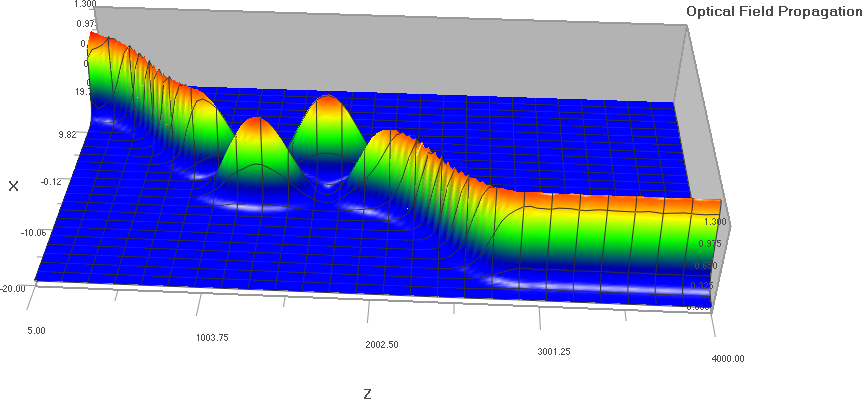
\includegraphics[width=0.7\textwidth]{Images/intensite900}
        \caption{Propagation à $\lambda_1=1.55\mu m$}
        \vspace*{1cm}
        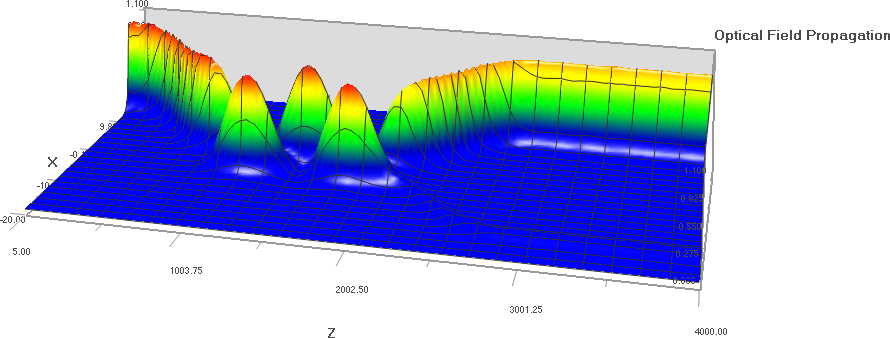
\includegraphics[width=0.7\textwidth]{Images/intensite900-2}
        \caption{Propagation à $\lambda_2=1.31\mu m$}
        \label{fig:}
    \end{center}
\end{figure}

%Est-ce que c'est swag ou pas ?
\section{Calculs d'isolation}
\begin{figure}[h]
    \begin{center}
\begin{tikzpicture}
\begin{axis}[width=0.6\textwidth,height=0.45\textwidth,
xmin=860, xmax=960,
ymin=0, ymax=60,
minor x tick num=1,
xlabel={Longueur des guides ($\mu m$)},
ylabel={Isolation (dB)},
legend columns=-1,
legend entries={$\lambda_1$, $\lambda_2$},
legend style={/tikz/every even column/.append style={column sep=0.5cm},at={(1,0.12)}}
]
\addplot table[x=Z, y=Isolation, col sep=comma, smooth]{../Isolation.csv};
\addplot table[x=Z, y=Isolation2, col sep=comma, smooth]{../Isolation.csv};
\end{axis}
\end{tikzpicture}
        \caption{Isolation des guides de sortie pour les deux longueurs d'onde}
        \label{big_graph}
    \end{center}
\end{figure}

On peut facilement obtenir une isolation au-delà de 20dB pour les deux longueurs d'ondes.

On remarque par ailleurs que les isolations peuvent atteindre jusqu'à 54dB, sans pour autant qu'on puisse obtenir de telles isolations sur un dispositif : il faut trouver un compromis entre les deux longueurs d'onde, ce qui nous empêche d'atteindre d'extrêmement bonnes isolations pour les deux longueurs d'onde à la fois.

La longueur optimale des guides sera alors de $916\mu m$, pour laquelle on atteint une isolation de 28dB pour les deux longueurs d'onde.


On peut supposer que pour d'autres longueurs de guides, on aura des pics d'isolation plus proches, et donc un fonctionnement plus optimal.\newline
La longueur de guides que nous avons choisie est néanmoins un bon compromis entre une bonne isolation, et un dispositif suffisamment compact pour être intégré dans des appareils où la contrainte de place est importante.«


%Isolation et Pertes
\chapter*{Conclusion}
\addcontentsline{toc}{chapter}{Conclusion}

Le démultiplexage est de nos jours très important et très largement utilisé dans les télécommunications. Comprendre son fonctionnement est primordial afin d'être capable d'en réaliser de plus complexes, pour de vraies applications.

Il est également important de connaître ses limites telles que celles que nous avons pu voir : le dimensionnement pour avoir la meilleure séparation possible, l'isolation qu'il faut optimiser au maximum pour éviter toute perte d'information, mais aussi la dépendance en longueur d'onde, le défaut de longueur d aux "S" d'entrée et de sortie qui prolongent le couplage.

Il faut aussi considérer les compromis à faire, par exemple entre la qualité d'isolation et la contrainte de place.

Tous ces éléments sont à considérer lorsque l'on veut réaliser un démultiplexeur. Les outils informatique dont nous disposons permettent de réaliser de nombreuses simulations afin d'adapter au mieux les paramètres avant de réaliser un travail de fabrication qui peut être lourd à mettre en place, ou du moins plus lourd qu'entrer un script et des valeurs puis lancer une simulation qui donnera tout autant, si ce n'est plus de résultats qu'une fabrication suivi d'une caractérisation. 

\nocite{*}
\bibliographystyle{unsrt}
\bibliography{Biblio}
\end{document}
